\begin{figure}
	\centering
		
	\hfill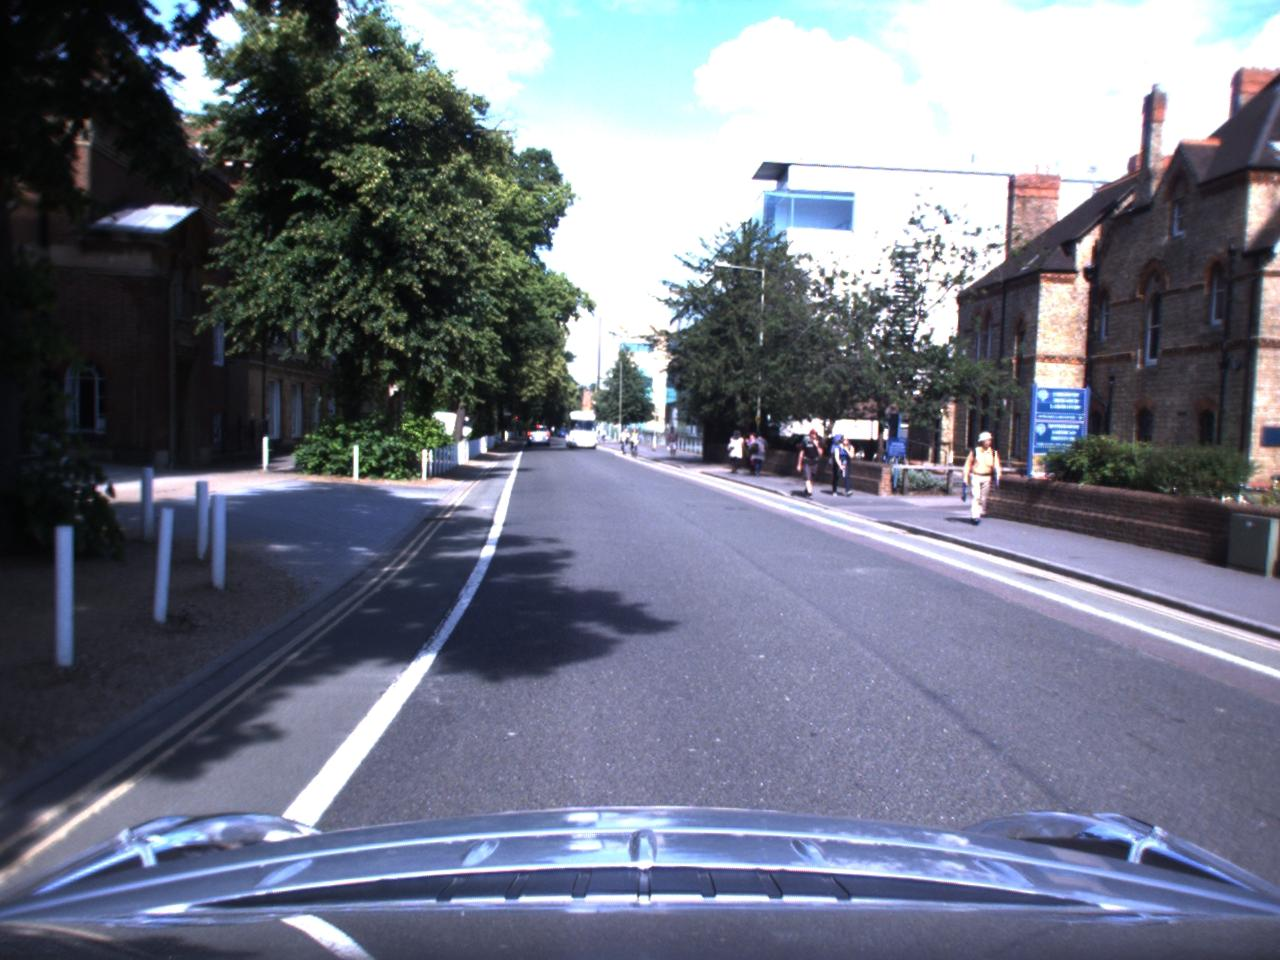
\includegraphics[width=0.25\linewidth]{preliminary/sun}\hfill
	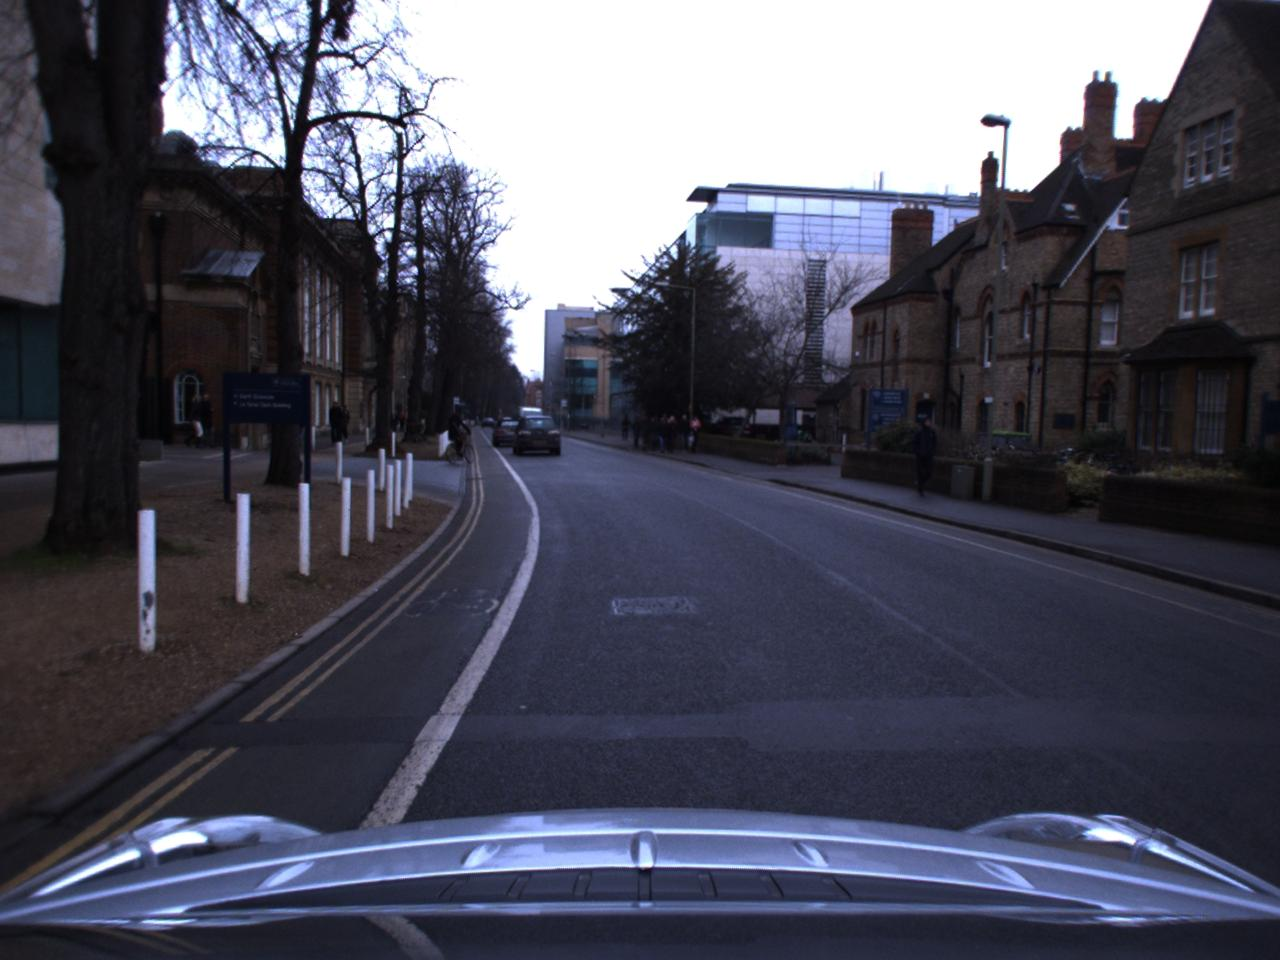
\includegraphics[width=0.25\linewidth]{preliminary/overcast}\hfill
	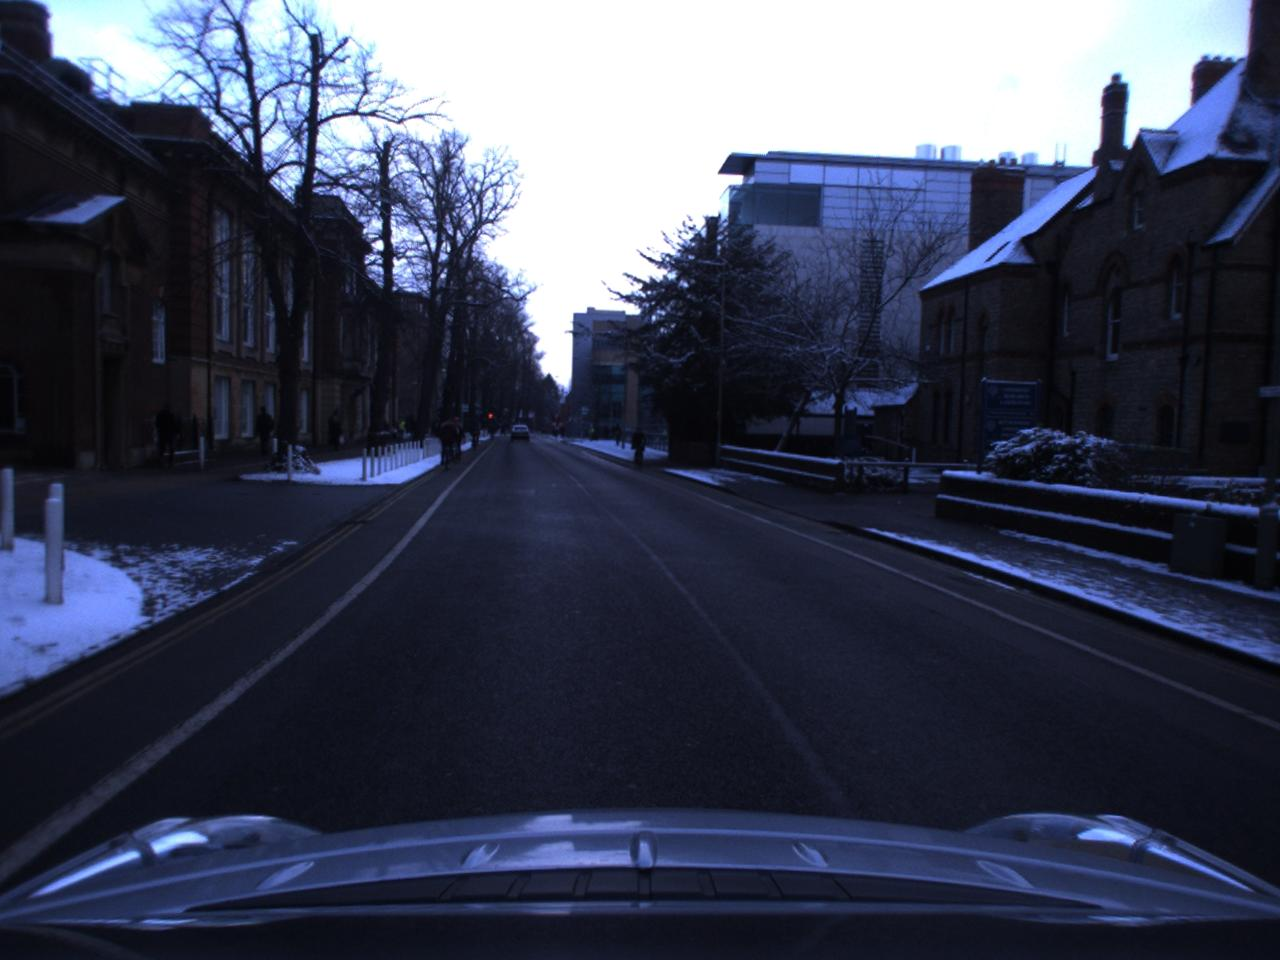
\includegraphics[width=0.25\linewidth]{preliminary/snow}\hfill
	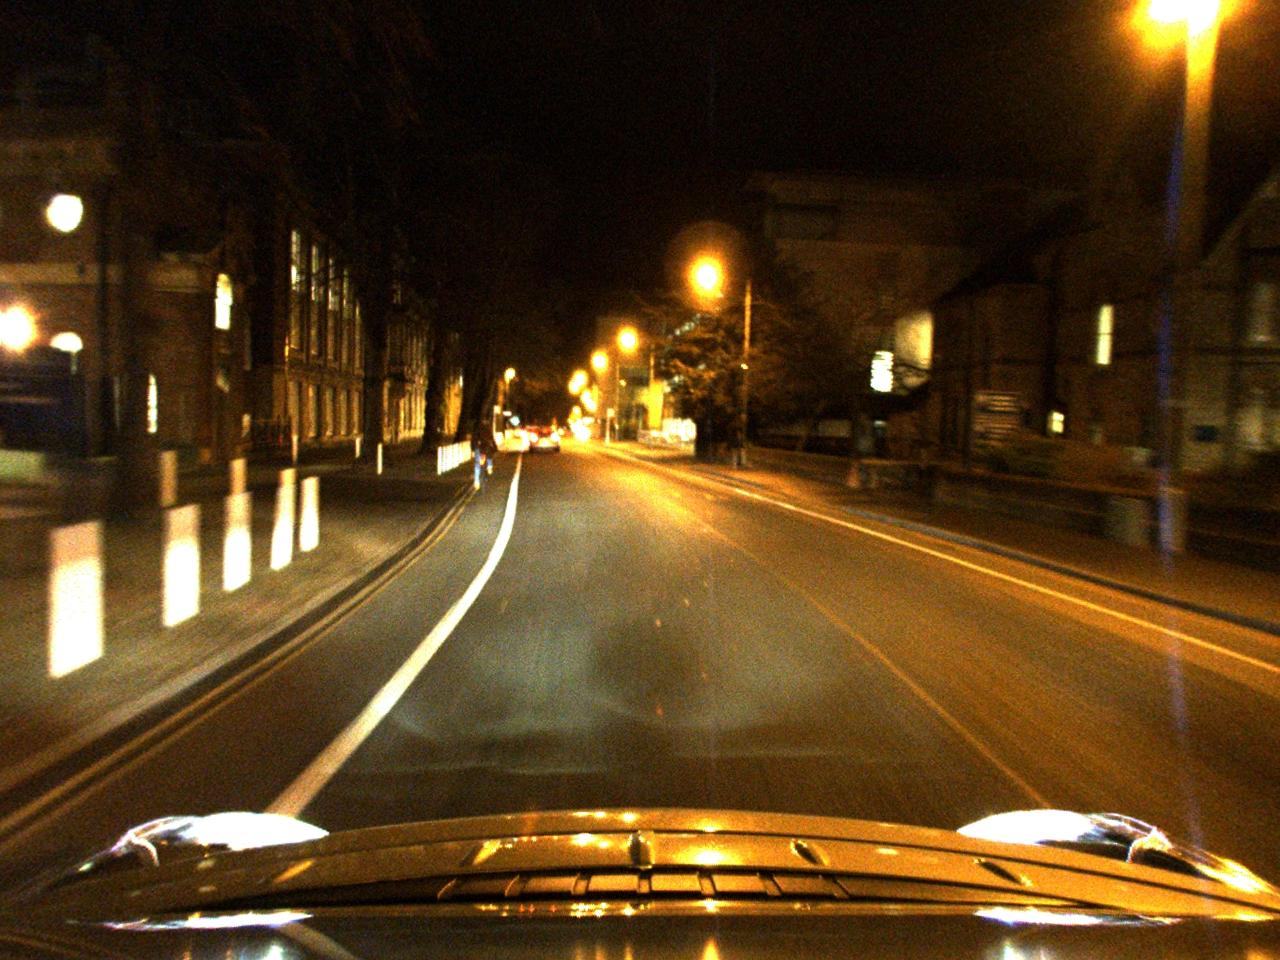
\includegraphics[width=0.25\linewidth]{preliminary/night}\hfill
	
	\hfill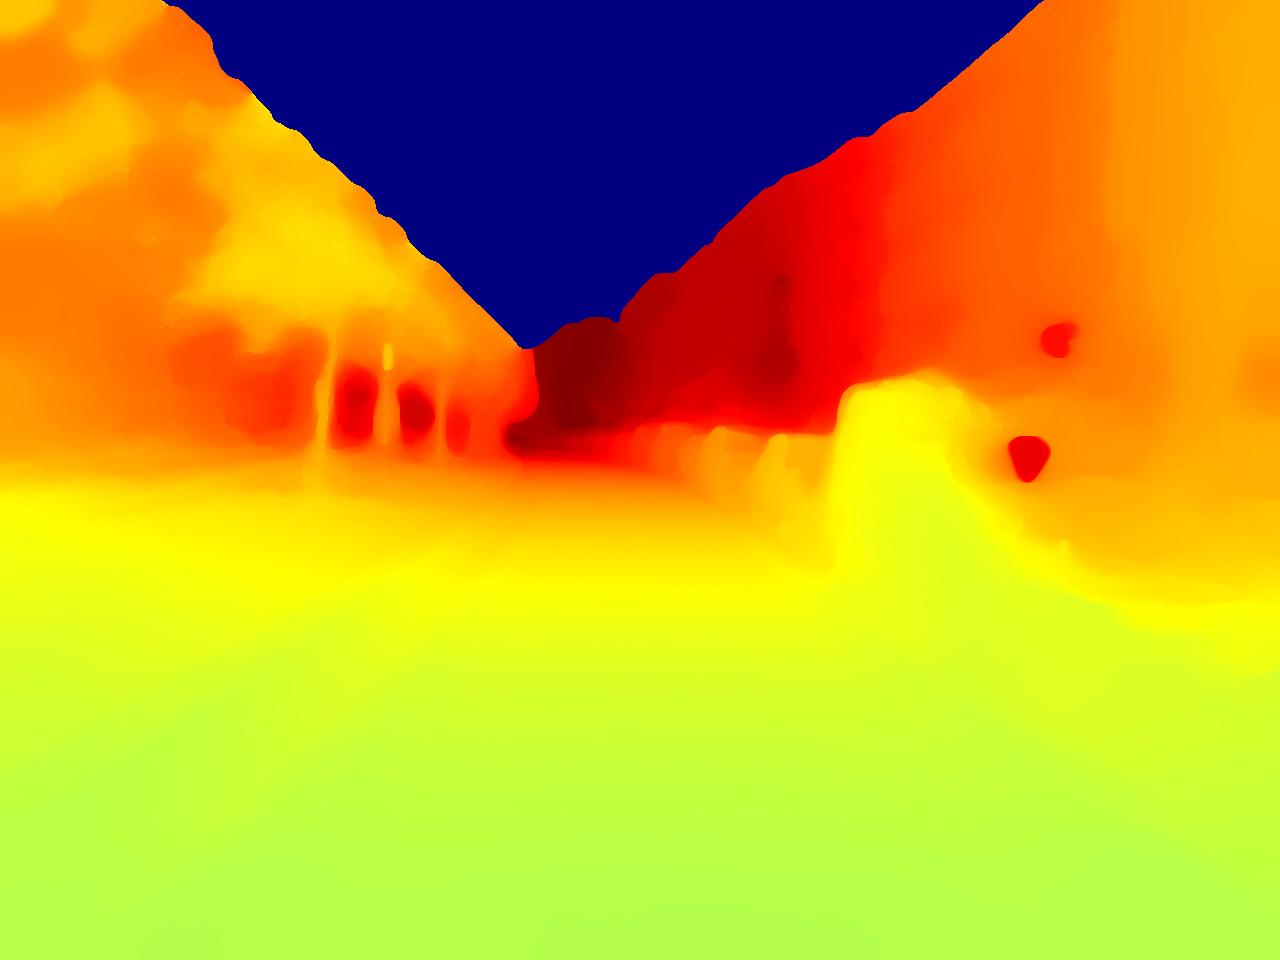
\includegraphics[width=0.25\linewidth]{preliminary/depth}\hfill
	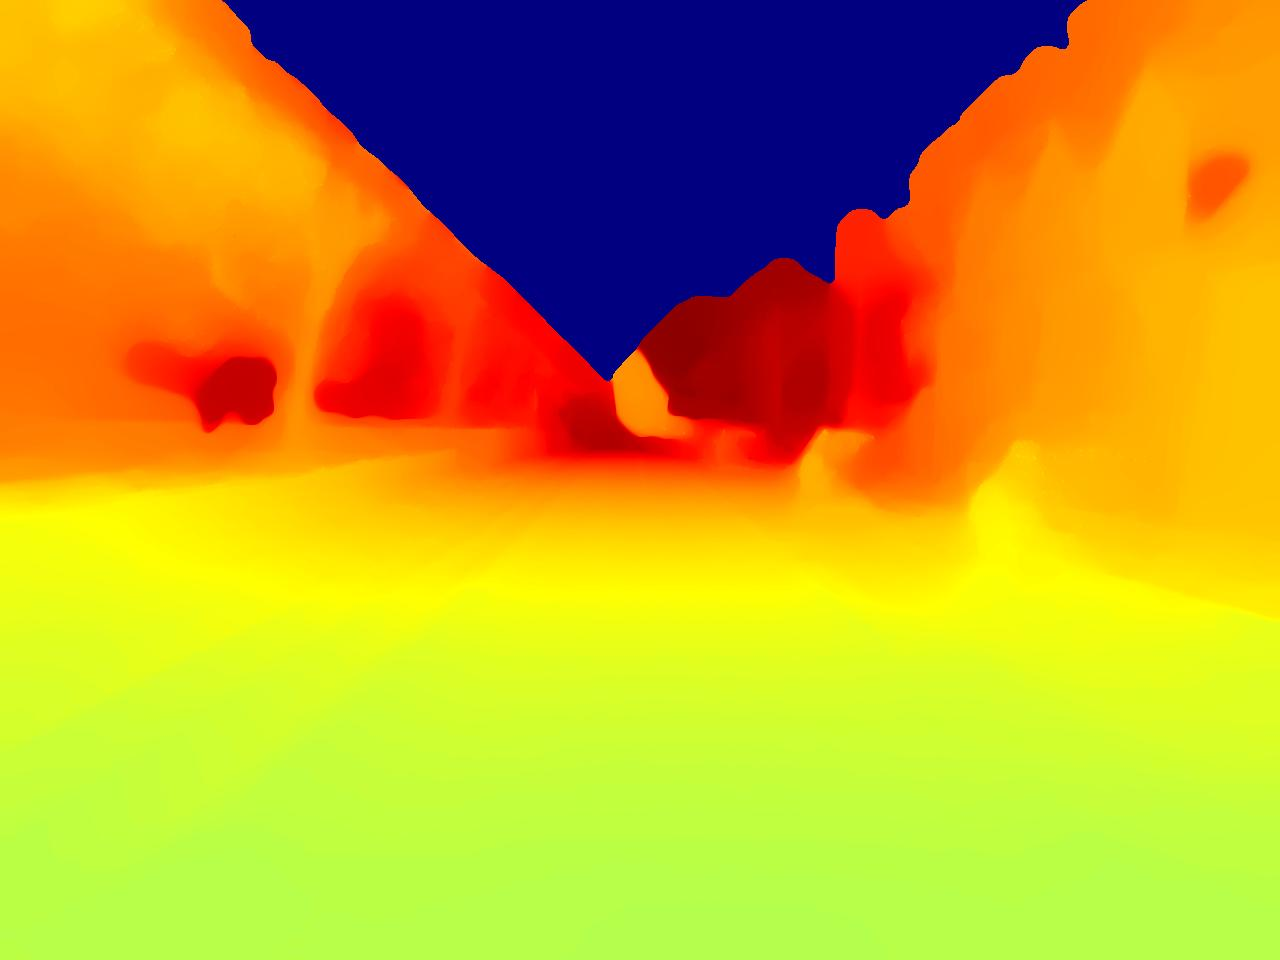
\includegraphics[width=0.25\linewidth]{preliminary/depth3}\hfill
	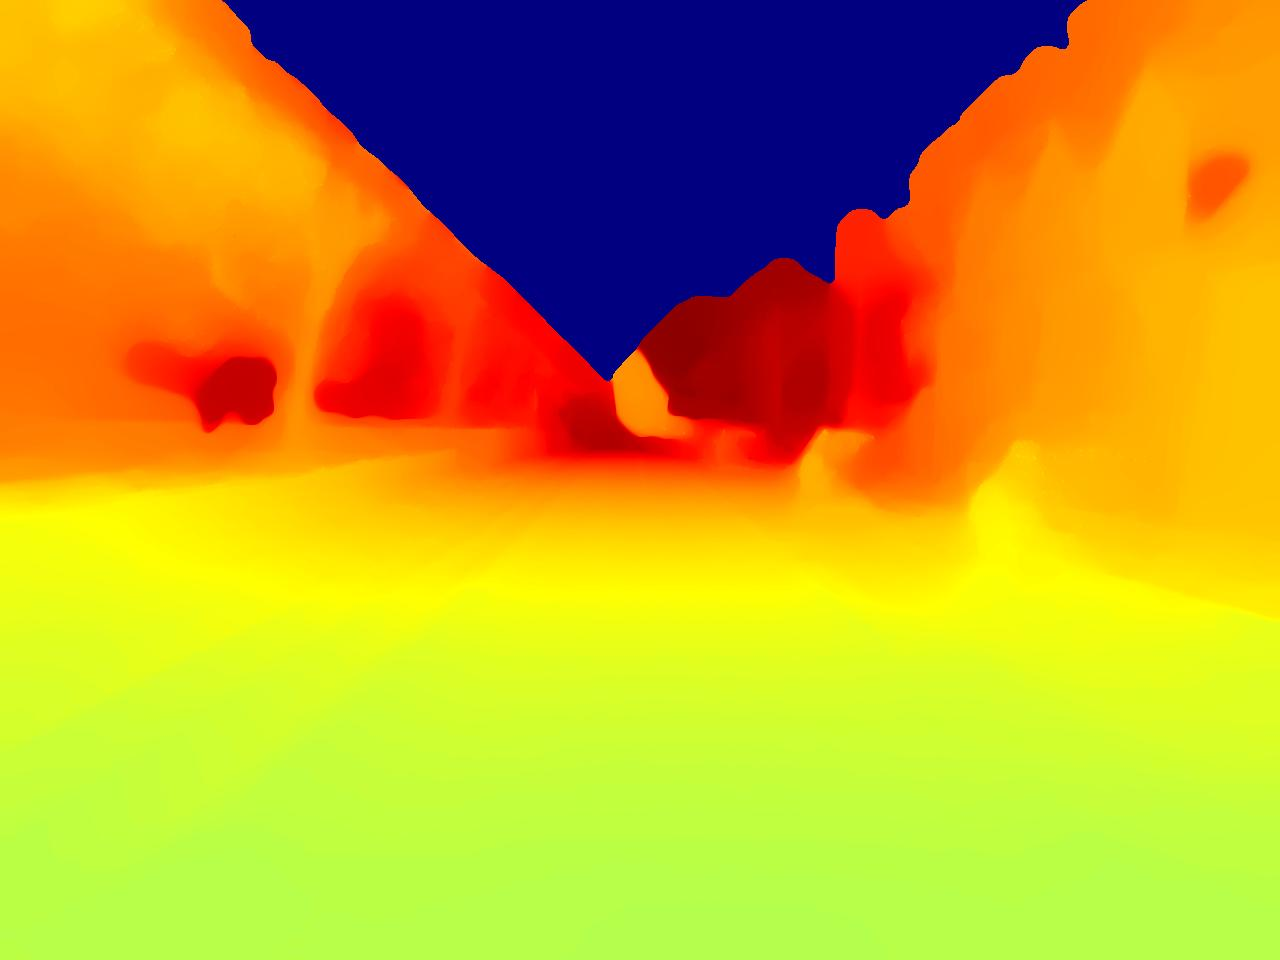
\includegraphics[width=0.25\linewidth]{preliminary/depth3}\hfill
	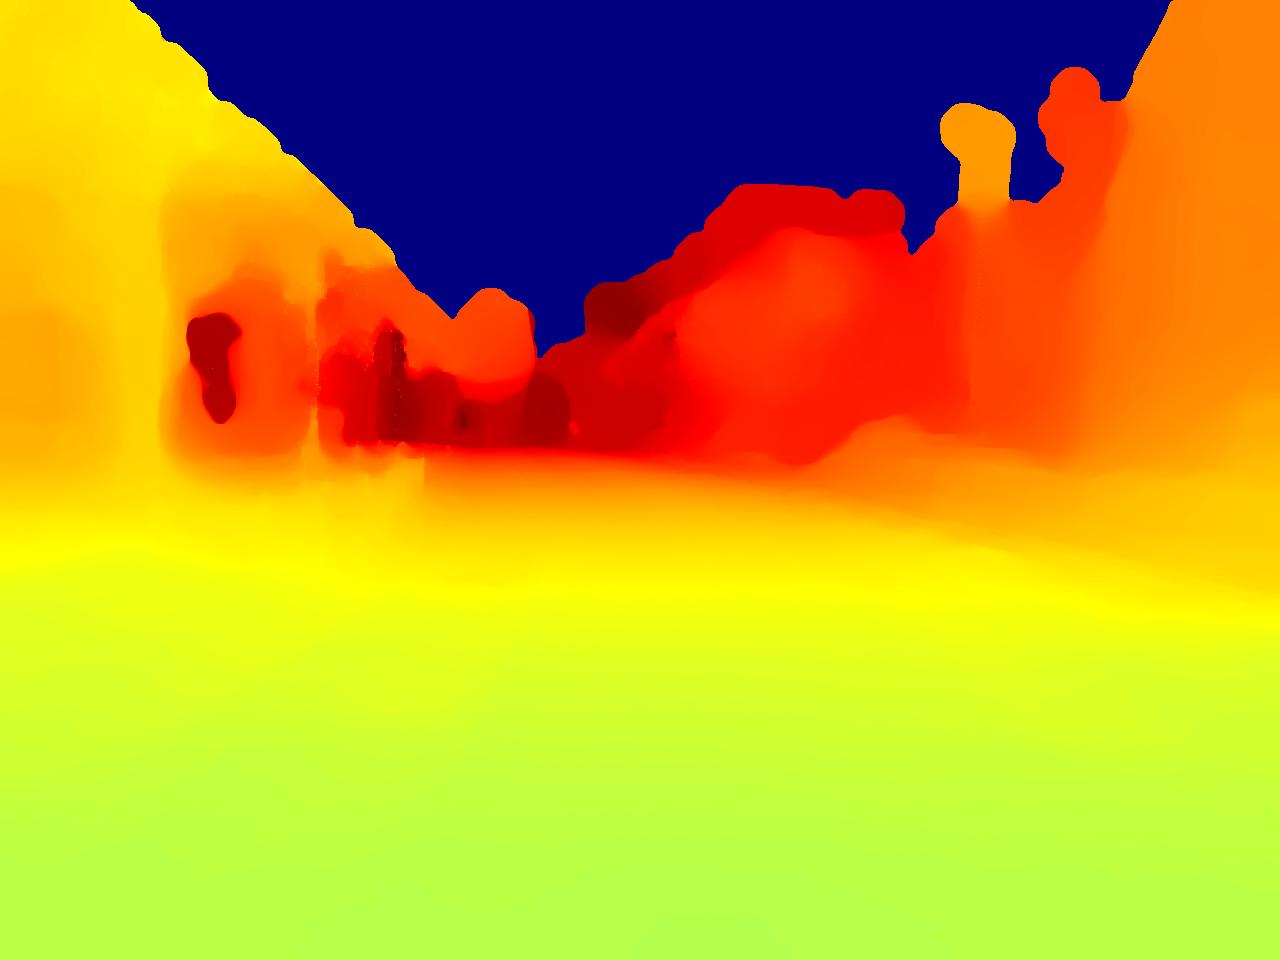
\includegraphics[width=0.25\linewidth]{preliminary/depth4}\hfill

	\caption[Images and depth maps comparison]{\label{fig:image_vs_depth} \textbf{Visual changes between radiometric and geometric domain:} due to outdoor conditions, visual aspect of images changes over time (top row), while, geometry of the scene (corresponding depth maps, bottom row) remains stable.}
	
\end{figure}
	